\hiddenref{}

\section{Introduction\label{introduction}}

\IEEEPARstart{U}{nique} personal identification using biometric characteristics is critical for the success of a range of e-governance programs, e-businesses and border security. Such automated capabilities to accurately establish personal identities have significantly increased the efficiency in e-governance programs and imparted enormous benefit to the citizens. Fingerprint is the oldest and one of the most widely used biometric. Millions of travelers around the world are required to provide their 4-4-2 fingerprints using slap-fingerprint devices which find their large-scale deployments, in most countries, China, India, USA or Brazil to name just a few, at the border crossing points. This is a mandatory requirement for most countries, either for enrollment in the national ID programs or for border crossings/entry, or both. Failure to acquire acceptable quality fingerprints is the key reason for user inconvenience that can be frequently observed at such imaging or user authentication facilities. Despite the significant success in the advancement and deployment of face recognition technologies today, fingerprint images continue to be acquired for large-scale applications, e.g. national ID programs or passport assisted border crossings. This can be attributed to the relative stability of this biometric due to aging, expression, or make-up changes and due to the fact that large-scale applications require multiple pieces of biometrics to more reliably establish the identity of individuals. When we register our fingerprint samples on various fingerprint acquisition devices, our finger knuckle patterns are inherently exposed and can be conveniently acquired. This can be quite convenient for both the user and the recipient of the data, as the fingerprint data is collected along with the finger knuckle data. This is important in view of encouraging evidences on the uniqueness \cite{cappelli2010minutia} and stability \cite{kumar2014importance} of finger knuckle patterns.

\subsection{Related Work\label{relate-work}}
\subsubsection{Finger Knuckle Identification\label{relate-work-fk}} 
User identification using finger dorsal patterns has attracted a large amount of interest in the biometrics community. Such images have shown a range of applications in forensics and online applications. Reference \cite{joshi1998computer} is believed to have first investigated the potential of finger dorsal patterns in establishing user identities. In order to enhance user convenience, contactless images were later incorporated to ascertain user identification capabilities. Finger knuckle patterns exhibit creases and curves whose thickness, unlike those for the fingerprint, varies significantly. Therefore reference \cite{kumar2015recovering} investigates the extraction of minutiae features to match finger knuckle images. Several publications have investigated a range of spatial \cite{woodard2005finger}, \cite{sricharan2006knuckle}, \cite{kumar2009personal}, \cite{zhang2010online}, \cite{zhu2010multimodal}, and spectral domain \cite{aoyama2011finger} methods to accurately match finger knuckle images. Significant advances in the capabilities of deep neural networks has enabled state-of-art finger knuckle identification methods that have shown outperforming results over the conventional methods. In this context, FKIMNet \cite{thapar2019fkimnet} and FKNet \cite{cheng2020deep} have illustrated promising performance and motive for further development of deep neural based methods to accurately match knuckle images visible during slap fingerprint acquisitions. Reference \cite{jaswal2016knuckle} provides an interesting summary of the range of finger knuckle identification methods introduced in the literature. 


\subsubsection{Fingerprint Identification\label{realate-work-fp}}
The choice of any specific fingerprint acquisition technique, among a range of widely available FBI-compliant \footnote[1]{Several national ID programs use FBI complaint sensors, for example, Aaadhaar program acquired 4-4-2 fingerprint images from over a billion of Indian residents using such \cite{fbi-sensor} slap-fingerprint sensors.} sensors \cite{fbi-sensor}, depends on the cost and intended nature of applications. In this context, the slap-fingerprint scanners are capable of acquiring multiple fingerprint impressions at the same time and therefore are widely deployed for civilian and border crossing applications. There are several factors that can limit the effectiveness of fingerprint images acquired from such fingerprint sensors for identity verification. Some of these limiting factors are: (a) cuts and bruises on fingers, (b) the presence of dirt or leftover impressions on the sensor, (c) environmental factors that cause dry and wet fingerprints, (d) aging factors from the epidermis, and (e) deformations resulting from the finger elasticity. Limitations of existing slap fingerprint segmentation algorithms are also known to degrade fingerprint matching accuracy and such degradation has also been articulated in NIST report \cite{watson2009slapssegii} and several references \cite{maltoni2009handbook}, \cite{zhang2010slap}.

Researchers have explored a variety of fingerprint matching techniques, using minutiae templates, or the combination of minutiae and texture features, and other alternative methods for matching fingerprint images \cite{maltoni2009handbook}. Among various state-of-the-art fingerprint matchers, the NBIS \cite{watson2007user} is an open-source fingerprint matcher provided by NIST. This matcher uses two key modules, namely MINDTCT and BOZORTH for the minutiae detection and template matching respectively. It is open source, complies with several standards, and is widely employed in a range of law-enforcement applications. The minutiae cylinder code (MCC) \cite{cappelli2010minutia} is widely considered as another state-of-the-art fingerprint matcher available in the public domain. Among various commercial off-the-shelf (COTS) matcher, the VeriFinger from Neurotechnology \cite{verifinger} is a widely used/deployed matcher and has known to offer higher matching accuracy. 


\begin{figure*}
    \centering
    \subfloat[]{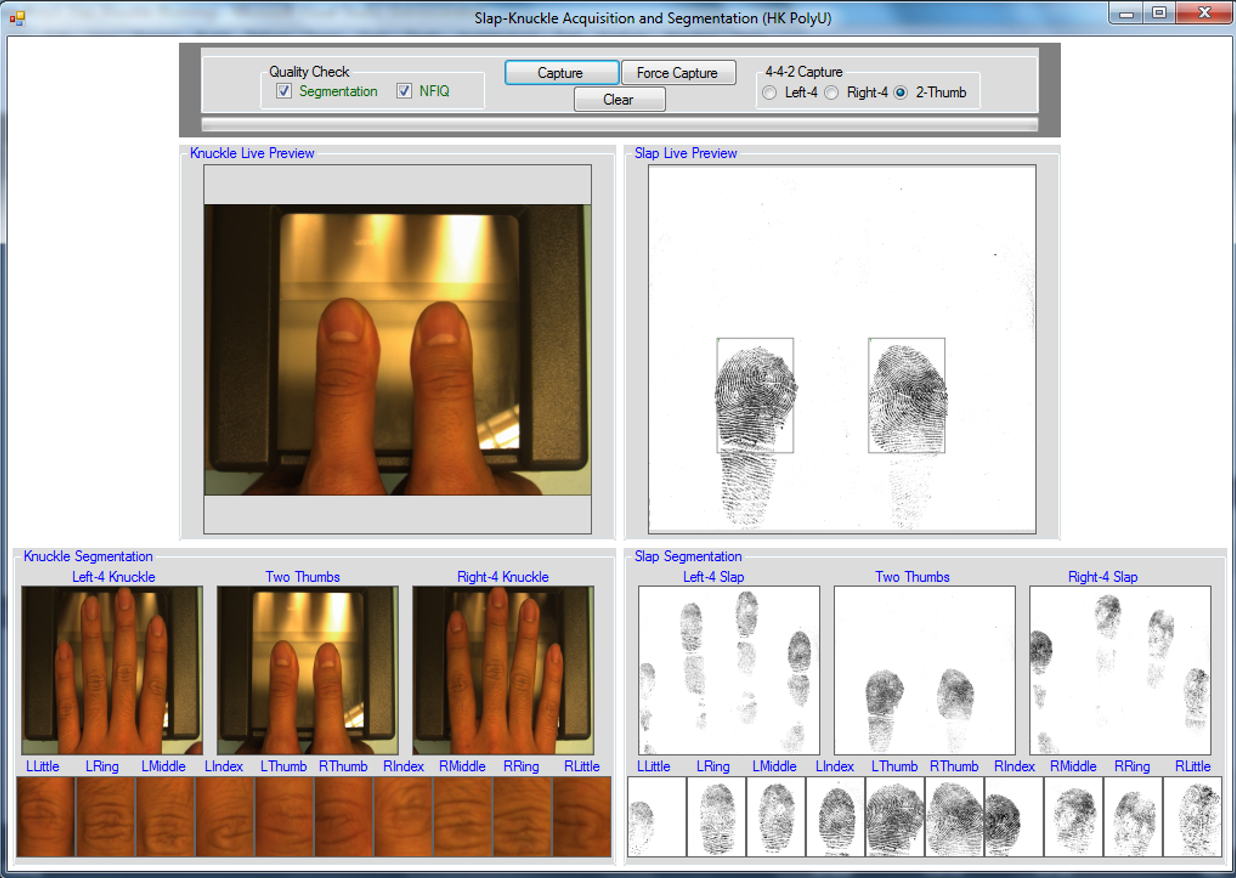
\includegraphics[width=4in]{Figures/system.png}%
    \label{system-a}}
    \hspace{0.1in}
    \subfloat[]{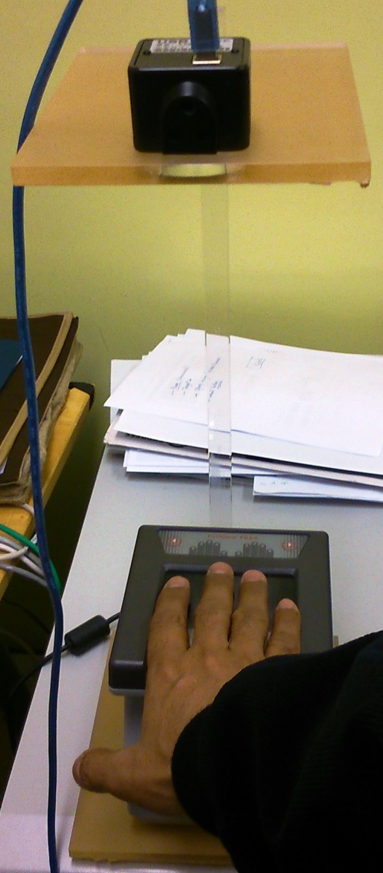
\includegraphics[width=1.250in]{Figures/system-sensor.png}%
    \label{system-sensor}}
    \caption{Online user authentication using slap-fingerprint and finger-knuckle images: (a) joint user interface developed for the 4-4-2 protocols (b) sensor placement for single shot imaging.}
    \label{system}
\end{figure*}

\subsection{Motivation and Our Work\label{motivation-contribution}}

The NIST report submitted to the US Congress \cite{2002SUMMARYON} underlines that about 2\% of the user population does not have usable fingerprints. NIST studies have also reported a false positive identification rate (FPIR) of ten-finger identification in the range of 1.5 to 3.5\% on a gallery size of about one million. Similar conclusions have also been reported in a large-scale proof-of-concept study undertaken by UIDAI \cite{uidai}. This study indicated that about 1.9\% of the subjects could not be reliably authenticated by only using their fingerprints. One of the critical challenges with large-scale deployed fingerprint authentication systems is also related to the acquisition of fingerprint images, and such sensing requires a fair degree of cooperation from the users. Therefore, it is not uncommon in the literature to report a failure to enroll (FTE) rate in the range of 1\% to 5\% for fingerprints. 

The drawback of currently popular fingerprint-only user identification can be complemented by incorporating finger knuckle information for user identification. Besides, there are several advantages of the new system. First, the data collection facility is easy to set with a low cost. Second, the data collection procedure is simple. Since the finger knuckle and fingerprint data can be collected simultaneously, no extra time is needed. Third, users will have almost the same user experience without any confusion. The key idea of this paper is to develop a finger-knuckle-assisted fingerprint identification system, as shown on the Fig. \ref{system}, to significantly improve user identification accuracy without causing additional user inconvenience. To achieve this goal, firstly, the fingerprint and finger knuckle data of each user must be acquired simultaneously and with a single imaging shot; secondly, both fingerprint and finger knuckle must be accurately segmented and aligned; finally, a dynamic fusion strategy must be introduced to accommodate degradation in the fingerprint and finger-knuckle quality and significantly enhance user the identification capabilities.

Convolution neural network can learn the robust features by updating the convolution kernels during backpropagation process, and we can use the CNN model to extract the knuckle pattern features. Such knuckle features are essentially texture features and represent low level features that may not need very deep CNN models recover. However, such CNN models don't \cite{jaderberg2015spatial} have rich rotational and translational invariance capabilities. During the presentation of slap-fingerprints, simultaneously visible knuckle creases are often deformed or translated the focus of subjects largely remains on finger tips to generate quality fingerprint impressions. Due to these factors, if we directly match the generated feature from CNN models, we can only achieve limited performance. Therefore, we introduce a new method to address such limitations with CNN by incorporating expected rotational and translational changes in such features and then using structural similarity index measure (SSIM) \cite{wang2004image} to compute more reliable match scores. 


The key contributions from this paper can be summarized as follows: 

\begin{itemize}
    \item This paper introduces a new biometric system, i.e. finger-knuckle-assisted fingerprint identification system in the Fig. \ref{system}, to address current limitations from widely deployed slap-fingerprint sensors at border crossings and national ID programs. This system simultaneously acquires fingerprint and finger knuckle images with a single imaging shot, with no additional user inconvenience or degradation in traffic flow, and can serve as an add-on system for the existing or the deployed slap fingerprint systems. Our research introduces more effective finger knuckle segmentation capabilities from the finger dorsal images acquired under complex backgrounds, ambient illumination, and in the present multiple finger knuckles that are inherently observed in such simultaneously acquired images. We incorporate dynamic fusion capabilities to address the limitations resulting from degraded fingerprint or finger-knuckle images. Our experimental results presented in this paper validate the effectiveness of the proposed biometric system for its usage in a range of real-world applications. 
    \item We develop the first joint finger-knuckle and fingerprint database, which has been acquired from 120 different subjects, using 4-4-2 imaging protocols, and introduced in the public domain. To the best of our knowledge, there is no such joint database developed or available so far, and its availability in the public domain will help to advance further research and development efforts for the real-applications. 
    \item We propose a new framework to accurately match finger knuckle patterns that are simultaneously acquired during a commercial slap fingerprint acquisition. This framework can more effectively accommodate rotational and translational changes in such knuckle patterns for generating accurate match scores (more details in Section \ref{fk-template}). We also present experimental results using several state-of-the-art finger knuckle matching methods to validate the effectiveness of the proposed method. 
\end{itemize}


The rest of this paper is organized as follows. Section \ref{fk-acquire} introduces a single-shot imaging-based framework for finger-knuckle-assisted slap fingerprint identification. This section also details the finger knuckle segmentation strategy developed to automatically segment finger knuckle images from the slap finger dorsal images acquired under complex and ambient imaging backgrounds. Section \ref{template-generation} introduces a dynamic scheme to consolidate finger knuckle and fingerprint match scores while Section \ref{experiment} presents the experimental results. Section \ref{discussion} presents a discussion and the key conclusions of this work are summarized in Section \ref{conclusion}.
